\subsubsection{Architektur}

Wie bei Swarm besteht Kubernetes aus zwei verschiedenen Arten von Knoten: den Master-Knoten und den Worker-Knoten.
Die Master Nodes werden auch Control Plane genannt und die Worker Nodes.
Ebenso wie in Swarm übernimmt der Master Node die Verwaltung des Clusters, während auf dem Worker Node die Container Engine läuft.

\begin{figure}[htbp]
\centering
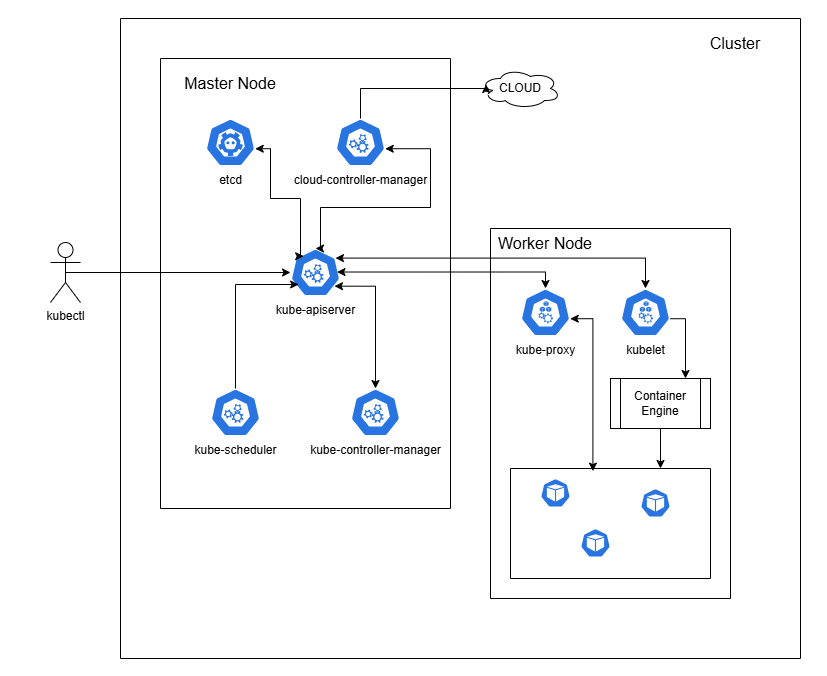
\includegraphics[width=0.8\textwidth]{bilder/grundlagen/kubernetes-architektur.png}
\caption{Kubernetes-Architektur}
\label{fig:kubernetes_architektur}
\end{figure}

Ein Master Node verfügt über einen kube-apiserver, der sowohl für die Kommunikation zwischen den Nodes als auch für die externe Kommunikation zuständig ist.
Über diesen steuert der Master Node den Cluster, d. h. er entscheidet auch darüber, ob neue Ressourcen angelegt oder überarbeitet werden. Der kube-apiserver kontrolliert, ob die Ressourcen, Limits und Quotas eingehalten werden.
Der kube-apiserver stellt auch die einzige Verbindung zur etcd-Datenbank im Master Node her. In der etcd-Datenbank stehen die Manifeste der Ressourcen des Clusters, daher ist dort auch der aktuelle Zustand des Clusters zu finden.
Auf dem Master Node befinden sich auch der Kube-Scheduler und der Kube-Controller-Manager, die für die Verwaltung des Clusters zuständig sind. Der Kubelet-Scheduler weiß, wie viel Ressourcen auf den Nodes und ihren Containern verbraucht werden und wie viel übrig sind.
Darüber hinaus steuert er das Pod-Scheduling, also die Verteilung der Pods auf den Nodes. Der kube-controller-manager übernimmt die Überwachung der laufenden Prozesse und reagiert auf Ereignisse. Beispielsweise verteilt er die Pods eines Nodes, der ausgefallen ist, auf die anderen Nodes.
Beide sind wiederum über den kube-apiserver erreichbar. Zu guter Letzt ist im Master Node auch der cloud-controller-manager enthalten, der die Kommunikation zu den Cloud-Diensten übernimmt und auch über die Cloud gesteuert werden kann, wenn der Cluster in einer Cloud betrieben wird.

Ein Cluster besteht auch üblich aus mehreren Worker Nodes. Diese übernehmen keine Verwaltung des Clusters sondern nur die Ausführung der Container. Dadurch sind die Worker Nodes austauschbar und  können auch ausfallen \parencite[vgl. 51]{welter2024kubernetes}. 
Auf dem Worker Node läuft die Controller Engine, die die Container betreibt.
In Kubernetes laufen die Container jedoch nicht direkt auf den Nodes, sondern in Pods, die auf den Nodes ausgeführt werden. Auf einem Node können mehrere Pods laufen.
Ein Worker Node besitzt ein Kubelet und einen Kube-Proxy. Letzteres verwaltet die Kommunikation zwischen den Pods und dem restlichen Netzwerk des Clusters. 
Das Kubelet verwaltet die Pods auf dem Worker Node. Es führt die Pods über die Controller Engine aus und überwacht diese.
Kubelet und Kube-Proxy sind direkt mit dem Kube-Apiserver von mindestens einem Master-Node verbunden. Der Kube-Apiserver beauftragt beispielsweise den Kubelet, einen Pod zu deployen. Dafür schickt er das Manifest des Pods an den Kubelet.
Ein Master Node hat ebenfalls ein Kubelet und einen Kube-Proxy, da zur Verwaltung des Clusters auch Pods auf ihm laufen. Der Master Node sollte jedoch nicht als zusätzlicher Worker Node genutzt werden.
\FloatBarrier